\section{Physical model}
\subsection{Coordinates, geometry, and droplet generation}
Let $Z$ denote the nominal downstream direction, $X$ the primary electrostatic-deflection direction, and $Y$ the substrate-transport direction. The droplet position and velocity are $\vect r_i=(X_i,Y_i,Z_i)$ and $\vect v_i$. Device geometry is represented by the external field and prescribed release, collection, exit and deposition surfaces in a common coordinate system.

The throw distance is the separation between the printhead exit and the substrate. Trajectories are evaluated at the deposition surface to determine the printed pattern, while clearance is assessed at the relevant collection and exit surfaces. The coordinate origin and surface locations are configuration inputs; the formulation applies independently of their particular values.

For an effective liquid-jet diameter $d_j$, frequency $f$, and wavelength $\lambda$, conservation of emitted liquid volume gives
\begin{align}
 U_j&=f\lambda, & \lambda&=\Lambda d_o,\\
 V_d&=\frac{\pi d_j^2\lambda}{4}, &
 d_d&=\left(\frac{3}{2}d_j^2\lambda\right)^{1/3}, &
 m_0&=\rho_l V_d.
\label{eq:drop}
\end{align}
Here $d_o$ is the nozzle-orifice diameter and $\Lambda$ is a prescribed wavelength-to-orifice ratio. The effective jet diameter need not equal the orifice diameter if contraction is independently characterized. We use $d_j=d_o$ in the consistent nominal example. The jet speed and airborne droplet diameter follow from Eq.~\eqref{eq:drop} for the selected nozzle and excitation parameters.

The calculation assumes one primary droplet per forcing cycle. It does not predict satellite production, breakup stability, the neck profile, or jet contraction. Liquid viscosity, surface tension, and modulation amplitude influence those processes, but are not solved by the present post-breakup particle model. They must not be described as resolved flight physics merely because they appear in a material-property record.

\subsection{Precomputed electrostatic field and particle coupling}
For specified electrode potentials and material permittivity, the continuum electrostatic problem is
\begin{equation}
 \nabla\cdot(\epsilon\nabla\phi)=-\rho_e,\qquad \vect E=-\nabla\phi.
\label{eq:field}
\end{equation}
The charge-free approximation is $\rho_e=0$ in the air domain. Electrode Dirichlet conditions, outer-boundary conditions, solid surfaces, and mesh resolution are part of the field problem. The field is evaluated once for each device geometry and electrode configuration. The implementation uses a finite-volume electrostatic solution exported from OpenFOAM. Mesh generation, electrode potentials, outer-boundary conditions, and export resolution define the reusable field model; they are held fixed during a raster search.

The particle code loads $\vect E$ on a regular Cartesian grid and uses trilinear interpolation:
\begin{equation}
 \vect E_h(\vect r)=\sum_{a,b,c\in\{0,1\}}
 w_a(\xi)w_b(\eta)w_c(\zeta)\vect E_{k+a,l+b,m+c},
 \quad w_0(s)=1-s,\;w_1(s)=s.
\end{equation}
The stored field has $N_X\times N_Y\times N_Z$ sample locations, with export spacings $\Delta X$, $\Delta Y$, and $\Delta Z$. These are \emph{export-grid spacings}, not a statement about the original unstructured-mesh resolution. The current interpolator returns zero outside the grid. A production assessment should instead flag an unintended domain exit; silently interpreting zero field as a physically justified continuation would be incorrect.

The imposed field is not updated in response to the droplets. Their mutual electrostatic interaction is calculated separately. Thus the model includes an imposed electrode field and direct particle interactions, but omits particle-induced image-charge corrections from conducting boundaries and a self-consistent particle--electrode Poisson solve.

\subsection{Command-to-charge conversion}
\subsubsection{Electronics, liquid resistance, and effective capacitance}
For a linear command calibration, a digital command $D_n$ requests
\begin{equation}
 V_{c,n}=\gamma D_n,\qquad \gamma=\frac{V_{\max}}{D_{\max}}.
\end{equation}
The voltage gain is $\gamma=V_{\max}/D_{\max}$ and the inverse gain is $\gamma^{-1}=D_{\max}/V_{\max}$. These ratios must not be interchanged.

The electrode voltage retains state across every physical droplet cycle:
\begin{equation}
 \tau_a\dot V_a+V_a=V_c(t),\qquad
 V_a(s)=V_{c,n}+(V_{a,n}^{0}-V_{c,n})e^{-s/\tau_a},
 \quad 0\leq s<T=1/f.
\label{eq:amp}
\end{equation}
The end-of-cycle voltage initializes the next cycle. Commands are held for a complete cycle; a guard or an unprinted logical slot is still an emitted droplet and an electronics-history event. The amplifier time constant is $\tau_a$, and charge is sampled at the prescribed breakup phase $t_b=\beta T$.

The effective resistance of a connected liquid column is approximated by a bulk segment and a narrow neck:
\begin{equation}
 R_l=\rho_{\mathrm{el}}
 \left[\frac{L_b-L_n}{\pi a_j^2}+\frac{L_n}{\pi a_n^2}\right],
 \quad L_n=\eta_n\lambda,\quad a_n=\eta_r(d_d/2),
\end{equation}
where $\rho_{\mathrm{el}}$ denotes electrical resistivity rather than mass density, and $L_b$ is the nozzle-to-breakup distance. These are fixed equivalent-circuit dimensions, not a resolved singular pinch-off geometry.

The software supports geometric capacitance estimates and a fitted driven capacitance $C_d$. The implemented parallel-plane and coaxial approximations are, respectively,
\begin{equation}
 C_{d,\mathrm{plane}}=\frac{2\pi\epsilon\lambda}
 {\operatorname{arcosh}(g/(2a_j))},\qquad
 C_{d,\mathrm{coax}}=\frac{2\pi\epsilon\lambda}{\ln(b/a_j)}.
\end{equation}
They are engineering approximations rather than a charging-electrode boundary-element solution. The liquid time constant uses
\begin{equation}
 C_\Sigma=C_d+C_r+C_s,\qquad \tau_l=R_l C_\Sigma.
\end{equation}
The driven capacitance governs equilibrium charge, whereas return and stray capacitances contribute to $\tau_l$. The electronics/cable load $C_{\mathrm{load}}$ is a different physical quantity; substituting it for the droplet--electrode capacitance would be unjustified. The effective $C_d$ is a calibrated parameter of the command-to-charge model rather than the measured electronics load.

\subsubsection{Mid-cycle charge and short-range induction}
Within each formation cycle the electrode-induced charge obeys
\begin{equation}
 \tau_l\dot q_e+q_e=-C_d V_a(t),\qquad q_e(0)=0.
\label{eq:liquid}
\end{equation}
The zero initial value is reset for each forming droplet. It is a modeling assumption: the implementation retains amplifier state and detached-neighbor charges, but not a continuous resolved liquid charge distribution. For $\tau_a\ne\tau_l$,
\begin{align}
 q_e(s)={}&-C_d V_{c,n}(1-e^{-s/\tau_l})\\
 &+C_d(V_{c,n}-V_{a,n}^{0})\frac{\tau_a}{\tau_a-\tau_l}
       (e^{-s/\tau_a}-e^{-s/\tau_l}).
\label{eq:charge_response}
\end{align}
The coincident-time-constant limit is evaluated analytically rather than by subtracting nearly equal exponentials.

The short-range detached-neighbor contribution is
\begin{equation}
 q_n=q_e(t_b)-\left(\kappa_1q_{n-1}+\kappa_2q_{n-2}\right)
                  (1-e^{-t_b/\tau_l}).
\label{eq:induction}
\end{equation}
The two preceding \emph{physical cycles}, including guards, enter this recurrence. The coefficients $(\kappa_1,\kappa_2)$ specify the selected charging-history closure. They parameterize a phenomenological charging-history closure motivated by guard-cancellation behavior. The closure represents the net effect of the preceding charge distribution without resolving a time-dependent electrode capacitance matrix. In-flight Coulomb forces are a separate process and are not replaced by these coefficients.

Explicit guard-voltage compensation is independently configurable. A first or second guard can request a fraction of the latest actual printed voltage; in the reported discovery case these fractions are zero. Zero guard command does \emph{not} imply zero detached guard charge when settling and induction are active. No additional consecutive-printed-drop voltage correction is applied in that case.

For specified net-charge targets, Eqs.~\eqref{eq:amp}--\eqref{eq:induction} are affine in the current command and can be inverted sequentially. The inversion must preserve guard commands and waveform state. Infeasible voltage requests are rejected, not silently clipped and presented as realized charge targets. Final feasibility is assessed by forward replay of quantized commands.

\subsection{Particle dynamics}
For each released, active droplet, the force balance is
\begin{equation}
 m_i\dot{\vect v}_i=
 m_i\vect g+q_i\vect E_h(\vect r_i)
 +\sum_{j\ne i}\vect F^{C}_{ij}
 +\vect F^D_i,\qquad \dot{\vect r}_i=\vect v_i.
\label{eq:motion}
\end{equation}
Additional specified body accelerations may be included. In the coupled coordinate convention, gravity acts along negative $Y$ in the current implementation. The charge of a detached droplet is constant between coalescence events; charge relaxation, ion exchange, and charge loss with evaporated solvent are not explicitly solved.

\subsubsection{Pairwise electrostatic interaction}
The monopole interaction is
\begin{equation}
 \vect F^{C}_{ij}=k_e q_iq_j
 \frac{\vect r_i-\vect r_j}{\|\vect r_i-\vect r_j\|^3}\,\chi_{ij}.
\label{eq:coulomb}
\end{equation}
The active-pair mask $\chi_{ij}$ excludes self-interactions and includes a configurable range cutoff. A finite interaction range $r_c$ or an all-pair setting can be selected. A small charge threshold is applied numerically. Near contact, the code suppresses this term when the squared center distance is not greater than $(1+\epsilon_c)(a_i+a_j)^2$, where $\epsilon_c$ is a prescribed near-contact tolerance. This switch prevents a singular point-particle force but is not a resolved near-contact electrohydrodynamic model. Its effect, and the range cutoff, require sensitivity tests.

The pair contribution is antisymmetric for an evaluated pair. This preserves equal-and-opposite internal electric forces, subject to roundoff and masks. It does not establish global momentum conservation once drag, gravity, evaporation, and imposed-field forces are included.

\subsubsection{Finite-Reynolds-number drag}
For carrier-air velocity $\vect u_i$ and slip $\vect w_i=\vect v_i-\vect u_i$,
\begin{align}
 \mathrm{Re}_i&=\frac{\rho_a(2a_i)\|\vect w_i\|}{\mu_a},\\
 \vect F^D_i&=-\frac{1}{2}\rho_a C_D(\mathrm{Re}_i)\pi a_i^2
                     \|\vect w_i\|\vect w_i,\\
 C_D(\mathrm{Re})&=
 \begin{cases}
 \dfrac{24}{\mathrm{Re}}(1+0.15\mathrm{Re}^{0.687}),&\mathrm{Re}<1000,\\
 0.44,&\mathrm{Re}\geq1000.
 \end{cases}
\label{eq:drag}
\end{align}
This is the implemented Schiller--Naumann form \citep{openfoamdrag}. Density, viscosity, and speed determine the local Reynolds number. The liquid droplet is treated as a sphere; internal circulation, deformation, lift, added mass, and the Basset history force are not separately represented.

\subsection{Aerodynamic wake and positive-air model}
\subsubsection{Nearest-upstream wake}
For target droplet $i$ and an ahead-of-target source $j$, define the positive trailing separation $\ell_{ij}=Z_j-Z_i$ and transverse separation $r_{\perp,ij}$. A source is eligible if
\begin{equation}
 \ell_{ij}\geq\alpha_{\min}a_j,\quad
 \ell_{ij}<L_{\max},\quad
 r_{\perp,ij}<b_{ij}=a_j+\ell_{ij}\tan\theta_w.
\end{equation}
The closest eligible source in axial distance is selected; wake velocities from all sources are not summed. With $U_j=|v_{Z,j}|$, the induced-air-speed fraction is
\begin{align}
 c_{ij}&=\min\left[c_{\max},\;\frac{\eta_w}{2}C_D(\mathrm{Re}_{j,Z})
                              \left(\frac{a_j}{b_{ij}}\right)^2\right],\\
 \vect u_{w,i}&=U_j c_{ij}
 \exp\left[-\gamma_w\left(\frac{r_{\perp,ij}}{b_{ij}}\right)^2\right]
 \frac{\vect v_j}{\|\vect v_j\|+\varepsilon}.
\end{align}
A second cap limits $\|\vect u_{w,i}\|$ to $c_{\max}|v_{Z,i}|$. The source Reynolds number uses its axial speed. The parameters $\alpha_{\min}$, $L_{\max}$, $\theta_w$, $\eta_w$, $\gamma_w$, and $c_{\max}$ define the axial support, spread, strength, radial decay and deficit cap.

The scaling is motivated by spreading a drag-associated momentum deficit over an expanding wake area. It is a reduced-order air-entrainment closure, not a solution of the wake momentum PDE, and it does not impose a global fluid momentum balance. ``Velocity deficit'' in the implementation describes the reduced slip experienced by a trailing droplet. The resulting induced air velocity is directed along the source motion.

\subsubsection{Mean positive-air coflow}
A specified positive-air volume flow $Q$ is mapped to an effective mean coflow:
\begin{equation}
 \overline{\vect u}_+=\eta_Q\frac{Q}{A_{\mathrm{eff}}}\vect e_Z.
\label{eq:positive_air}
\end{equation}
For $Q$ in L/min and $A_{\mathrm{eff}}$ in mm$^2$, explicit SI conversion is required. $A_{\mathrm{eff}}$ is an effective entrainment area, not necessarily a geometric port area, and $\eta_Q$ is a coupling efficiency. This relation does not compute pressure losses, wall boundary layers, or an actual manifold flow solution.

\subsubsection{Correlated fluctuations and coherent transverse motion}
The optional unsteady component uses $K$ spatial Fourier modes and independent stationary Ornstein--Uhlenbeck modal amplitudes:
\begin{align}
 A_{c,k}^{n+1}&=\rho_t A_{c,k}^n+\sqrt{1-\rho_t^2}\,\xi_{c,k}^n,
 &\rho_t&=e^{-\Delta t/\tau_c},\\
 u'_{+,c}(Z,t_n)&=s_Q\sigma_c\sqrt{\frac{2}{K}}
 \sum_{k=1}^{K} A_{c,k}^n\cos(k_k Z+\varphi_{c,k}),
 &s_Q&=Q/Q_{\mathrm{ref}}.
\label{eq:ou}
\end{align}
Here $c$ denotes a Cartesian component; $\xi$ is standard Gaussian, phases are fixed pseudorandom draws, and wavelengths are geometrically spaced between a reference correlation length and four times that length. The initialized modal amplitudes have unit variance. The normalization targets the intended amplitude in an ensemble sense, not exact samplewise variance at every point.

A coherent transverse term is
\begin{equation}
 \vect u_{\mathrm{coh}}=s_Q A_v
 \begin{bmatrix}\sin\psi\\\cos\psi\\0\end{bmatrix},
 \qquad \psi=2\pi f_v t+2\pi Z/L_c.
\end{equation}
This is a prescribed rotating crossflow pattern; it must not be interpreted as a resolved vortex or a no-slip CFD solution. The complete carrier velocity is
\begin{equation}
 \vect u_i=\vect u_{w,i}+\overline{\vect u}_++\vect u'_+(Z_i,t)+\vect u_{\mathrm{coh}}(Z_i,t).
\end{equation}
Disabling unsteadiness sets the fluctuating and coherent amplitudes to zero but retains mean coflow. Setting $Q=0$ removes all positive-air terms while retaining droplet-induced wakes.

For diagnostics the drag is decomposed exactly as
\begin{align}
 \vect F^D_i={}&\underbrace{\mathcal D(\vect v_i)}_{\text{still-air drag}}
 +\underbrace{\mathcal D(\vect v_i-\vect u_{w,i})-\mathcal D(\vect v_i)}_{\text{wake correction}}\\
 &+\underbrace{\mathcal D(\vect v_i-\vect u_{w,i}-\vect u_{+,i})
                  -\mathcal D(\vect v_i-\vect u_{w,i})}_{\text{positive-air correction}},
\end{align}
where $\mathcal D$ is Eq.~\eqref{eq:drag}. The differences telescope, so the wake is not counted a second time as an independent empirical force. The corrections are directed and nonlinear, not pairwise momentum-conserving forces.

\begin{figure}[htbp]
\centering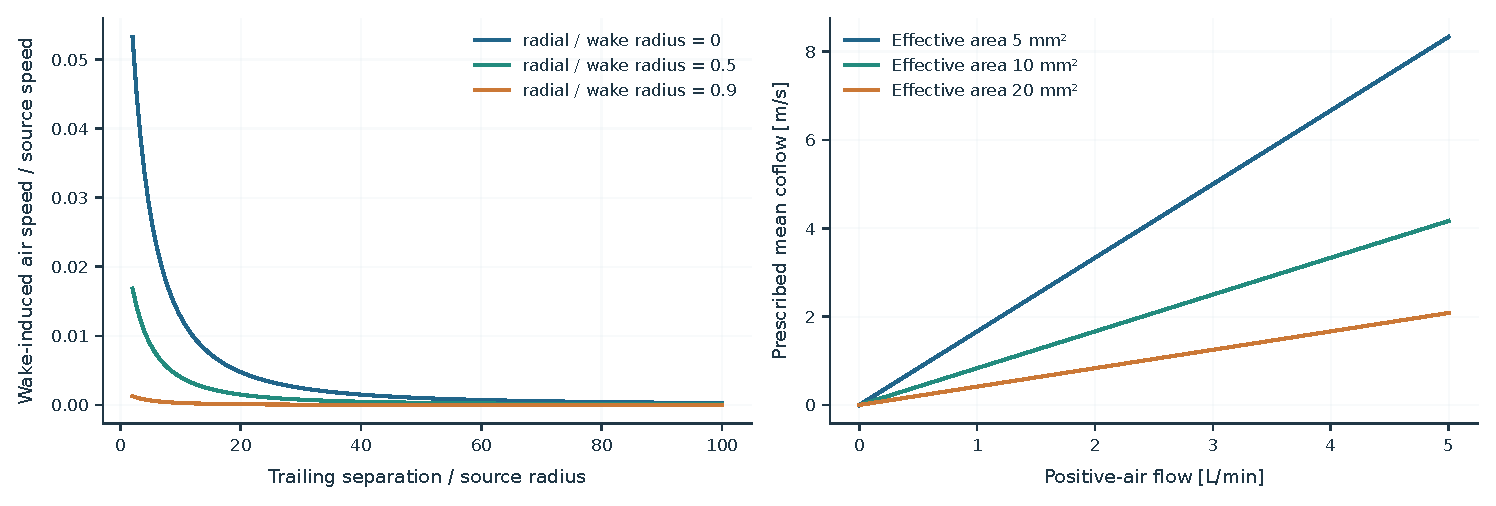
\includegraphics[width=\linewidth]{figures/aerodynamic_closures.pdf}
\caption{Behavior of the implemented engineering closures. Left: wake-induced air speed for three transverse offsets. Right: mean coflow from prescribed volume flow for different effective areas at $\eta_Q=0.5$. These are equation evaluations, not measurements or new CFD results. Positive-air robustness is not demonstrated by the zero-flow discovery case.}
\end{figure}

\subsection{Mass evolution and contact}
\subsubsection{Empirical distance-dependent mass loss}
The integrator decreases droplet mass using
\begin{equation}
 m_i^{n+1}=\max\left[m_i^n-k_m|v_{Z,i}^n|\Delta t
                   \left(\frac{a_i^n}{a_0}\right)^2,m_{\mathrm{floor}}\right],
 \qquad a_i=\left(\frac{3m_i}{4\pi\rho_l}\right)^{1/3}.
\end{equation}
The coefficient $k_m$ specifies the initial mass lost per unit axial travel. This is an empirical mass-loss closure, rather than a thermodynamic evaporation model. Temperature, vapor concentration, latent heat, solvent composition, and charge carriage by vapor are not evolved. Its applicability is bounded by the characterized ink and operating conditions.

\subsubsection{Contact detection and merge lineage}
A merge candidate is identified when
\begin{equation}
 \|\vect r_i-\vect r_j\|\leq(1-\delta_c)(a_i+a_j),\qquad 0\leq\delta_c<1.
\end{equation}
Deterministic greedy pairing allows each particle to merge at most once in a time step. The lower-index survivor inherits total mass and charge, mass-weighted position and velocity, and the union of lineage IDs. The radius follows the combined volume at fixed density. This approximates perfectly inelastic merging; it does not model bouncing, film drainage, droplet deformation, or surface-energy-mediated breakup.

A consequential implementation limit is that merge eligibility follows the intended-print mask. In common two-stroke adapters only the current requested targets are eligible; neutral guards and previous-stroke particles still influence forces, but are not generally eligible for permanent merging. Therefore a reported zero merge count means \emph{no detected merge among eligible targets under this rule}, not proof that every physical collision is absent.
